\chapter[Planteamientos]{Planteamientos}
% \label{cp:introduction}

{
\parindent0pt


% \textit{Official Repository: \href{https://github.com/joseareia/ipleiria-thesis}{GitHub Repository}}

\vspace{.935em}

\section{Problema 1 (25\%)}

\subsection{Literal a}
Aplicando Criptoanálisis por factorización, especifique el proceso y determine el PlainText (P) del siguiente Criptograma RSA (puede usar WolframAlpha para funciones exponenciales):

\begin{itemize}[leftmargin=*]
    \item $p=19$, $q=67$
    \item $KU=(5,1273)$
    \item Criptograma: $1252-1079-319-337-231-1100-507-1100-231-213-192$
\end{itemize}

\textbf{Algoritmo AEE (n, a):}
\begin{lstlisting}[basicstyle=\ttfamily]
Hacer (g0, g1, u0, u1, v0, v1, i) = (n, a, 1, 0, 0, 1, 1)
Mientras gi distinto 0 hacer
    Hacer yi+1 = parte entera (gi-1/gi)
    Hacer gi+1 = gi-1 - yi+1 × gi
    Hacer ui+1 = ui-1 - yi+1 × ui
    Hacer vi+1 = vi-1 - yi+1 × vi
    Hacer i = i+1
Si (vi-1 < 0)
    Hacer vi-1 = vi-1 + n
Hacer x = vi-1
\end{lstlisting}




\textbf{Solución:}


Se nos proporciona la siguiente información:

\begin{itemize}
\item $n = 1273$
\item $p = 19$
\item $q = 67$
\item $d = 5$
\item $z = (p-1)(q-1) = (19-1)(67-1) = 1188$
\end{itemize}

Y el siguiente mensaje cifrado:

\begin{verbatim}
1252 1079 319 337 231
1100 507 1100 231 213
192
\end{verbatim}

\subsubsection{Cálculo del inverso multiplicativo módulo $z$}

Necesitamos encontrar $e$ tal que $e \cdot d \equiv 1 ~mod~z$, es decir, el inverso multiplicativo de $d$ módulo $z$.

Para ello utilizaremos el algoritmo de Euclides extendido:

\textbf{Inicialización del algoritmo:}

Estamos buscando $e$ tal que $e \cdot 5 \equiv 1 ~\text{mod}~{1188}$

Inicializamos las variables según el algoritmo:

$$g_0 = 1188, g_1 = 5$$
$$u_0 = 1, u_1 = 0$$
$$v_0 = 0, v_1 = 1$$



\textbf{Iteración 1:}

Calculamos $y_2 = \lfloor g_0 / g_i \rfloor = \lfloor 1188 / 5 \rfloor = 237$

Calculamos $g_2 = g_0 - y_2 \cdot g_i = 1188 - 237 \cdot 5 = 3$

Calculamos $u_2 = u_0 - y_2 \cdot u_i = 1 - 237 \cdot 0 = 1$

Calculamos $v_2 = v_0 - y_2 \cdot v_i = 0 - 237 \cdot 1 = -237$



\textbf{Iteración 2:}

Calculamos $y_3 = \lfloor g_1 / g_i \rfloor = \lfloor 5 / 3 \rfloor = 1$

Calculamos $g_3 = g_1 - y_3 \cdot g_i = 5 - 1 \cdot 3 = 2$

Calculamos $u_3 = u_1 - y_3 \cdot u_i = 0 - 1 \cdot 1 = -1$

Calculamos $v_3 = v_1 - y_3 \cdot v_i = 1 - 1 \cdot -237 = 238$



\textbf{Iteración 3:}
Calculamos $y_4 = \lfloor g_2 / g_i \rfloor = \lfloor 3 / 2 \rfloor = 1$

Calculamos $g_4 = g_2 - y_4 \cdot g_i = 3 - 1 \cdot 2 = 1$

Calculamos $u_4 = u_2 - y_4 \cdot u_i = 1 - 1 \cdot -1 = 2$

Calculamos $v_4 = v_2 - y_4 \cdot v_i = -237 - 1 \cdot 238 = -475$



\textbf{Iteración 4:}

Calculamos $y_5 = \lfloor g_3 / g_i \rfloor = \lfloor 2 / 1 \rfloor = 2$

Calculamos $g_5 = g_3 - y_5 \cdot g_i = 2 - 2 \cdot 1 = 0$

Calculamos $u_5 = u_3 - y_5 \cdot u_i = -1 - 2 \cdot 2 = -5$

Calculamos $v_5 = v_3 - y_5 \cdot v_i = 238 - 2 \cdot -475 = 1188$



\textbf{Resultado final:}

El algoritmo ha terminado porque $g_4 = 0$

El inverso se encuentra en el valor de $v$ en el penúltimo paso: $v_3 = -475$

Como $v_3 < 0$, ajustamos: $v_3 = v_3 + B = -475 + 1188 = 713$

Por lo tanto, el inverso multiplicativo de 5 módulo 1188 es 713

Verificación: $5 \cdot 713 \equiv 1 ~\text{mod}~1188$

\begin{table}[h]
\centering
\begin{tabular}{|c|c|c|c|c|}
\hline
$i$ & $y_i$ & $g_i$ & $u_i$ & $v_i$ \\ \hline
0 & - & 1188 & 1 & 0 \\ \hline
1 & - & 5 & 0 & 1 \\ \hline
2 & 237 & 3 & 1 & -237 \\ \hline
3 & 1 & 2 & -1 & 238 \\ \hline
4 & 1 & 1 & 2 & -475 \\ \hline
5 & 2 & 0 & -5 & 1188 \\ \hline
\end{tabular}
\caption{Cálculo del inverso modular utilizando el algoritmo de Euclides extendido}
\label{tab:euclides}
\end{table}

Por lo tanto $e = 713$.

\subsubsection{Descifrado del mensaje}

Para descifrar el mensaje, utilizamos la fórmula $M = C^e ~\text{mod}~ n$, donde $e = 713$ y $n = 1273$.

\subsubsection{Proceso de descifrado}

$C = 1252: M = 1252^{713} ~\text{mod}~ 1273 = 80$ (ASCII: 'P')

$C = 1079: M = 1079^{713} ~\text{mod}~ 1273 = 117$ (ASCII: 'u')

$C = 319: M = 319^{713} ~\text{mod}~ 1273 = 98$ (ASCII: 'b')

$C = 337: M = 337^{713} ~\text{mod}~ 1273 = 108$ (ASCII: 'l')

$C = 231: M = 231^{713} ~\text{mod}~ 1273 = 105$ (ASCII: 'i')

$C = 1100: M = 1100^{713} ~\text{mod}~ 1273 = 99$ (ASCII: 'c')

$C = 507: M = 507^{713} ~\text{mod}~ 1273 = 97$ (ASCII: 'a')

$C = 1100: M = 1100^{713} ~\text{mod}~ 1273 = 99$ (ASCII: 'c')

$C = 231: M = 231^{713} ~\text{mod}~ 1273 = 105$ (ASCII: 'i')

$C = 213: M = 213^{713} ~\text{mod}~ 1273 = 111$ (ASCII: 'o')

$C = 192: M = 192^{713} ~\text{mod}~ 1273 = 110$ (ASCII: 'n')

\begin{table}[h]
\centering
\begin{tabular}{|c|c|c|}
\hline
$C$ & $M$ & ASCII \\ \hline
1252 & 80 & 'P' \\ \hline
1079 & 117 & 'u' \\ \hline
319 & 98 & 'b' \\ \hline
337 & 108 & 'l' \\ \hline
231 & 105 & 'i' \\ \hline
1100 & 99 & 'c' \\ \hline
507 & 97 & 'a' \\ \hline
1100 & 99 & 'c' \\ \hline
231 & 105 & 'i' \\ \hline
213 & 111 & 'o' \\ \hline
192 & 110 & 'n' \\ \hline
\end{tabular}
\caption{Descifrado RSA: $m = c^e ~\text{mod}~ n$}
\label{tab:descifrado}
\end{table}

\subsubsection{Mensaje descifrado}

El mensaje descifrado es:

\begin{verbatim}
Publicacion
\end{verbatim}





\pagebreak
\subsection{Literal b}
¿En qué principios \textit{(al menos 2)} reposa la seguridad de RSA?

\textbf{Respuesta:}
\begin{itemize}
    \item La gran dificultad computacional que hay inscrita en el problema de la factorización de números enteros grandes.
    \item La complejidad del problema del logaritmo discreto.
    \item La función de una vía con trampa (trapdoor) que permite cifrar fácilmente pero descifrar solo con información "privilegiada".
\end{itemize}

\subsection{Literal c}
¿Por qué la Criptografía de Curvas Elípticas es una opción viable para los retos Crypto actuales?

\textbf{Respuesta:}

En efecto maestro, la Criptografía de Curvas Elípticas (ECC) es una opción viable porque:
\begin{itemize}
    \item Ofrece el mismo nivel de seguridad que el RSA pero ya con claves de un menor tamaño.
    \item Hay menor consumo de recursos computacionales.
    \item Tiene una mayor eficiencia en dispositivos con recursos limitados.
    \item Presenta mayor resistencia a los ataques cuánticos en comparación con RSA.
\end{itemize}

\section{Problema 2 (25\%)}

\subsection{Literal a}
En el marco de la Seguridad Ofensiva, describa la secuencia para verificar y explotar una vulnerabilidad de acceso remoto a un host (tipo Win o Linux) y describa alguna estrategia de uso en un proceso de "Hacking Ético".


\textbf{Respuesta:}
La secuencia para verificar y explotar una vulnerabilidad de acceso remoto sigue un proceso metodológico conocido como "Cyber Kill Chain" o ciclo de ataque, que en el contexto de hacking ético permite identificar, evaluar y documentar vulnerabilidades de forma sistemática:

\begin{enumerate}
    \item \textbf{Obtención de Información (Reconocimiento):} 
    \begin{itemize}
        \item Recopilación de datos sobre el objetivo mediante técnicas OSINT.
        \item \textit{Herramientas:} Usenet, whois, dig, nslookup, dnsmap, fierce, DNSPredict.
        \item Enfoque ético: Limitarse a fuentes públicas y obtener autorización previa.
    \end{itemize}

    \item \textbf{Escaneo:} 
    \begin{itemize}
        \item Identificación de hosts activos, puertos abiertos y servicios en ejecución.
        \item Detección de sistemas operativos y versiones de software.
        \item \textit{Herramientas:} Fping, hping, nmap, SuperScan, AutoScan, xprobe2, Nessus.
        \item Enfoque ético: Realizar escaneos en horarios de bajo impacto y con notificación previa.
    \end{itemize}

    \item \textbf{Enumeración:} 
    \begin{itemize}
        \item Obtención de usuarios, grupos, recursos compartidos y configuraciones.
        \item \textit{Herramientas:} DumpSec, NmbSscan, Telnet, NetCat, rpcinfo, snmpenum.
        \item Enfoque ético: Documentar meticulosamente cada hallazgo sin explotar información sensible.
    \end{itemize}

    \item \textbf{Obtención de Acceso:} 
    \begin{itemize}
        \item Explotación de vulnerabilidades identificadas para obtener acceso inicial.
        \item \textit{Herramientas:} Airsnarf, dsniff, Metasploit Framework.
        \item Enfoque ético: Limitar el impacto de la explotación y documentar cada acción.
    \end{itemize}

    \item \textbf{Escalamiento de Privilegios:} 
    \begin{itemize}
        \item Elevación de permisos para obtener control administrativo del sistema.
        \item \textit{Herramientas:} John the Ripper, LCP, rcrack, ophcrack, Cain\&Abel, Metasploit Framework.
        \item Enfoque ético: Utilizar técnicas que no comprometan la estabilidad del sistema.
    \end{itemize}

    \item \textbf{Hurto o Exfiltración de Información:} 
    \begin{itemize}
        \item Simulación de extracción de datos sensibles para demostrar el impacto.
        \item \textit{Herramientas:} Rhosts, Config Files, Cain \& Abel.
        \item Enfoque ético: No extraer datos reales; utilizar marcadores o datos de prueba.
    \end{itemize}

    \item \textbf{Cubrimiento de Pistas:} 
    \begin{itemize}
        \item Análisis de logs y rastros digitales.
        \item \textit{Herramientas:} Logclean-ng, wtmpclean, rootkits, dataflows.
        \item Enfoque ético: Documentar todas las modificaciones realizadas para facilitar la restauración.
    \end{itemize}

    \item \textbf{Creación de Puertas Traseras:} 
    \begin{itemize}
        \item Demostración de cómo un atacante podría mantener acceso persistente.
        \item \textit{Herramientas:} Cron, Register Keys, Netcat, psexec, keyloggers, fwpclnt.dll, ps, netstat.
        \item Enfoque ético: Eliminar completamente cualquier puerta trasera al finalizar las pruebas.
    \end{itemize}
\end{enumerate}

\textbf{Estrategia de uso en un proceso de Hacking Ético:}

Una estrategia efectiva para implementar estas fases en un proceso de hacking ético incluye:

\begin{itemize}
    \item \textbf{Definición clara del alcance:} Establecemos los límites específicos y objetivos de la evaluación mediante un acuerdo formal (Rules of Engagement).
    
    \item \textbf{Enfoque de caja negra, gris o blanca:} Adaptamos la metodología según el nivel de información previa disponible sobre el objetivo.
    
    \item \textbf{Documentación exhaustiva:} Registramos meticulosamente cada paso, herramienta, hallazgo y recomendación para facilitar la remediación.
    
    \item \textbf{Prueba de concepto (PoC) controlada:} Demostramos las vulnerabilidades con impacto mínimo y sin afectar operaciones críticas.
    
    \item \textbf{Comunicación continua:} Mantenemos informados a los responsables del sistema, especialmente ante hallazgos críticos que requieran atención inmediata.
    
    \item \textbf{Análisis de impacto:} Evaluamos cada vulnerabilidad en función de la criticidad, facilidad de explotación e impacto potencial en el negocio.
    
    \item \textbf{Recomendaciones priorizadas:} Proporcionamos soluciones que sean prácticas y priorizamos la mitigación de esas vulnerabilidades encontradas.
\end{itemize}

Con este enfoque podemos identificar y documentar vulnerabilidades de forma sistemática, proporcionando una base sólida para mejorar la postura de seguridad de la organización.





\subsection{Literal b}
Enumere al menos 3 controles (de un estándar, normativa o Sistema de Gestión de Seguridad de la Información), que puedan implementarse posterior a un proceso de Seguridad Ofensiva, como estrategia preventiva.

\textbf{Respuesta:}

\begin{enumerate}
    \item \textbf{ISO/IEC 27001:2013 - Anexo A}
    \begin{itemize}
        \item \textbf{A.12.6.1 Gestión de las vulnerabilidades técnicas}: Este control requiere que se obtenga información oportuna sobre vulnerabilidades técnicas de los sistemas de información, se evalúe la exposición de la organización a dichas vulnerabilidades y se tomen medidas apropiadas para abordar los riesgos asociados.
        
        \textit{Aplicación post-seguridad ofensiva}: Tras un pentesting o evaluación ofensiva, este control permite establecer un proceso sistemático para abordar las vulnerabilidades descubiertas, priorizarlas según su criticidad e implementar las correcciones necesarias. Incluye la creación de un inventario preciso de activos tecnológicos, la suscripción a servicios de alertas de vulnerabilidades y la implementación de procedimientos regulares de parcheo.
        
        \item \textbf{A.9.4.2 Procedimientos seguros de inicio de sesión}: Establece que el acceso a los sistemas y aplicaciones debe estar controlado por procedimientos seguros de inicio de sesión.
        
        \textit{Aplicación post-seguridad ofensiva}: Después de que las pruebas de intrusión revelen debilidades en los mecanismos de autenticación, este control impulsa la implementación de técnicas robustas como limitación de intentos fallidos, registro detallado de accesos, tiempo de espera para sesiones inactivas, y no mostrar identificadores de sistema hasta que el proceso de inicio de sesión se haya completado exitosamente.
        
        \item \textbf{A.13.1.3 Segregación en redes}: Indica que los grupos de servicios de información, usuarios y sistemas deben estar segregados en redes diferentes.
        
        \textit{Aplicación post-seguridad ofensiva}: Cuando las evaluaciones de seguridad revelan problemas de movimiento lateral o elevación de privilegios, este control permite implementar arquitecturas de red segmentadas con firewalls internos, zonas desmilitarizadas (DMZ) y redes VLAN separadas por funciones, limitando el impacto potencial de una brecha de seguridad.
    \end{itemize}

    \item \textbf{NIST SP 800-53 Rev. 5}
    \begin{itemize}
        \item \textbf{SI-7 Integridad del software, firmware y la información}: Requiere que la organización emplee herramientas para detectar cambios no autorizados en software, firmware e información.
        
        \textit{Aplicación post-seguridad ofensiva}: Tras identificar manipulaciones o inyecciones durante pruebas ofensivas, este control permite implementar mecanismos de verificación de integridad como sumas de comprobación, firmas digitales y monitoreo en tiempo real para detectar alteraciones no autorizadas en archivos críticos del sistema o aplicaciones.
        
        \item \textbf{AC-6(1) Privilegio mínimo - Autorizar acceso a funciones de seguridad}: Especifica que la organización debe autorizar explícitamente el acceso a funciones específicas de seguridad y a información relacionada con la seguridad.
        
        \textit{Aplicación post-seguridad ofensiva}: Cuando las pruebas revelan exceso de privilegios o controles de acceso débiles, este control permite implementar una estrategia rigurosa de privilegio mínimo, separando cuentas administrativas de cuentas regulares, empleando sistemas de gestión de acceso privilegiado (PAM) y requiriendo autorizaciones específicas para acceder a funciones de seguridad críticas.
        
        \item \textbf{SC-7(10) Protección de límites - Prevenir tráfico saliente no autorizado}: Requiere que el sistema de información impida la exfiltración no autorizada de información.
        
        \textit{Aplicación post-seguridad ofensiva}: Después de que las pruebas de penetración revelen canales potenciales de exfiltración de datos, este control permite implementar sistemas de prevención de pérdida de datos (DLP), monitoreo avanzado de tráfico de red, inspección de SSL/TLS y filtrado de contenido saliente para prevenir la fuga de información sensible.
    \end{itemize}

    \item \textbf{CIS Controls v8}
    \begin{itemize}
        \item \textbf{Control 6.7 - Gestionar vulnerabilidades en dispositivos de red}: Gestionar vulnerabilidades para todos los dispositivos de red en uso en la empresa.
        
        \textit{Aplicación post-seguridad ofensiva}: Cuando las evaluaciones revelan debilidades en infraestructura de red, este control permite implementar escaneos regulares de vulnerabilidades específicos para dispositivos de red, monitoreo de configuraciones inseguras, y procesos automatizados para actualizar firmware y aplicar parches a routers, switches y firewalls.
        
        \item \textbf{Control 3.3 - Configurar el registro de auditoría}: Requiere configurar el registro para sistemas operativos, servidores, estaciones de trabajo, dispositivos de red y aplicaciones.
        
        \textit{Aplicación post-seguridad ofensiva}: Tras detectar actividades maliciosas durante las pruebas, este control permite implementar un sistema centralizado de gestión de logs (SIEM) con capacidades avanzadas de correlación y alertas, configurando registros detallados para eventos críticos de seguridad, intentos de autenticación fallidos, cambios de configuración y accesos a información sensible.
        
        \item \textbf{Control 4.1 - Establecer y mantener un proceso de gestión de configuraciones seguras}: Establece un proceso para administrar configuraciones seguras.
        
        \textit{Aplicación post-seguridad ofensiva}: Cuando un ejercicio de red team revela configuraciones débiles, este control permite implementar líneas base de seguridad automatizadas, herramientas de gestión de configuración y verificación continua contra plantillas de reforzamiento (hardening templates) para sistemas operativos, aplicaciones, servicios en la nube y dispositivos de red.
    \end{itemize}

    \item \textbf{OWASP ASVS 4.0 (Application Security Verification Standard)}
    \begin{itemize}
        \item \textbf{V2.2.1 - Verificación de contraseñas}: Requiere que todas las contraseñas de usuario sean almacenadas con algoritmos de hashing suficientes usando salt o con una funcionalidad criptográfica clave, con factores de trabajo (retrasos) apropiados.
        
        \textit{Aplicación post-seguridad ofensiva}: Después de que pruebas ofensivas revelen vulnerabilidades en almacenamiento de credenciales, este control permite implementar algoritmos modernos de hashing como Argon2id, bcrypt o PBKDF2 con factores de trabajo ajustables, adicionando salt únicos para cada contraseña y asegurando que no existan contraseñas almacenadas en texto plano o con hashing débil.
        
        \item \textbf{V5.3.5 - Validación de entradas}: Especifica que la aplicación debe sanitizar, deshabilitar o sandbox contenido HTML, CSS y JavaScript proporcionado por el usuario.
        
        \textit{Aplicación post-seguridad ofensiva}: Tras descubrir vulnerabilidades de inyección durante pruebas de penetración, este control permite implementar bibliotecas de validación/sanitización, configurar cabeceras de seguridad como Content-Security-Policy, y utilizar técnicas avanzadas como listas blancas para filtrar entradas de usuario y prevenir ataques como XSS, CSRF y clickjacking.
    \end{itemize}

    \item \textbf{PCI DSS 3.2.1}
    \begin{itemize}
        \item \textbf{Requisito 11.5}: Implementar mecanismos de detección de cambios (como herramientas de monitoreo de integridad de archivos) para alertar al personal sobre modificaciones no autorizadas de archivos críticos del sistema, archivos de configuración o contenido.
        
        \textit{Aplicación post-seguridad ofensiva}: Cuando las pruebas de seguridad revelan manipulaciones de archivos o configuraciones, este control permite implementar soluciones de monitoreo de integridad de archivos (FIM) que generan alertas en tiempo real ante cambios no autorizados en binarios de sistema, archivos de configuración, contenido web y carpetas críticas.
        
        \item \textbf{Requisito 6.6}: Para aplicaciones web públicas, abordar nuevas amenazas y vulnerabilidades continuamente y asegurar que estas aplicaciones estén protegidas contra ataques conocidos mediante revisiones manuales o automáticas de aplicaciones, instalando un firewall de aplicación web o ambas opciones.
        
        \textit{Aplicación post-seguridad ofensiva}: Después de identificar vulnerabilidades web en pentesting, este control permite implementar Web Application Firewalls (WAF) con reglas personalizadas basadas en las vulnerabilidades específicas encontradas, complementado con escaneos dinámicos de aplicaciones (DAST) y revisiones de código automatizadas (SAST) como parte del ciclo de desarrollo continuo.
    \end{itemize}
\end{enumerate}

Estos controles abarcan las diversas capas de seguridad \textit{(red, aplicación, sistema)} y provienen de estándares ampliamente reconocidos en la industria. Ya su implementación surge como una estrategia preventiva posterior a procesos de seguridad ofensiva permite construir un programa de seguridad sólido y basado en las vulnerabilidades reales identificadas durante las pruebas.




\subsection{Literal c}
Cómo puede obtenerse más información de una vulnerabilidad, describa la estructura básica que se expone en los repositorios de las mismas.

\textbf{Respuesta:}

Los repositorios de vulnerabilidades como NVD (National Vulnerability Database), CVE (Common Vulnerabilities and Exposures), MITRE, o Exploit-DB proporcionan información estructurada y detallada sobre vulnerabilidades de seguridad. Para obtener información completa sobre una vulnerabilidad específica, es fundamental comprender la estructura estandarizada que estos repositorios utilizan.

\subsubsection{Estructura básica de repositorios de vulnerabilidades}

\begin{itemize}
    \item \textbf{Identificador único (CVE-ID):} Formato CVE-YYYY-NNNNN que identifica unívocamente cada vulnerabilidad (ej. CVE-2021-44228 para Log4Shell).
    
    \item \textbf{Descripción técnica:} Explicación detallada del problema, incluyendo el tipo de vulnerabilidad (desbordamiento de búfer, inyección SQL, XSS, etc.).
    
    \item \textbf{Sistemas afectados:} Productos, versiones y configuraciones vulnerables mediante CPE (Common Platform Enumeration).
    
    \item \textbf{Métricas de severidad CVSS:} Sistema matemático de puntuación que cuantifica la gravedad de la vulnerabilidad.
    
    \item \textbf{Evaluación de impacto:} Consecuencias potenciales en términos de confidencialidad, integridad y disponibilidad.
    
    \item \textbf{Referencias técnicas:} Enlaces a informes de investigación, pruebas de concepto y avisos de seguridad.
    
    \item \textbf{Mitigaciones:} Soluciones o estrategias para abordar la vulnerabilidad (parches, configuraciones, etc.).
    
    \item \textbf{Metadatos temporales:} Fechas de descubrimiento, publicación, actualización y parche.
    
    \item \textbf{CWE (Common Weakness Enumeration):} Clasificación del tipo de debilidad de seguridad subyacente.
\end{itemize}

\subsubsection{Sistema CVSS - El modelo matemático de evaluación}

El Common Vulnerability Scoring System (CVSS) es un componente crucial de los repositorios modernos que proporciona un marco matemático para cuantificar objetivamente la gravedad de las vulnerabilidades. La versión actual (CVSS v3.1) utiliza un modelo matemático complejo basado en:

\begin{itemize}
    \item \textbf{Métricas Base:} Características intrínsecas e inmutables de la vulnerabilidad.
    \begin{itemize}
        \item \textit{Métricas de Explotabilidad:} Cuantifican la facilidad de explotación.
        \begin{itemize}
            \item Vector de Ataque (AV): ¿Cómo se explota? Red (0.85), Adyacente (0.62), Local (0.55), Físico (0.2).
            \item Complejidad de Ataque (AC): ¿Qué tan difícil es explotar? Baja (0.77), Alta (0.44).
            \item Privilegios Requeridos (PR): ¿Qué nivel de acceso necesita el atacante? Ninguno (0.85), Bajo (0.62/0.68), Alto (0.27/0.5).
            \item Interacción del Usuario (UI): ¿Se requiere participación del usuario? Ninguna (0.85), Requerida (0.62).
        \end{itemize}
        
        \item \textit{Métricas de Impacto:} Cuantifican el daño potencial.
        \begin{itemize}
            \item Alcance (S): ¿La vulnerabilidad afecta a otros componentes? Sin Cambio (U), Cambiado (C).
            \item Confidencialidad (C): Impacto en la protección de datos. Alto (0.56), Bajo (0.22), Ninguno (0).
            \item Integridad (I): Impacto en la fiabilidad de los datos. Alto (0.56), Bajo (0.22), Ninguno (0).
            \item Disponibilidad (A): Impacto en la accesibilidad. Alto (0.56), Bajo (0.22), Ninguno (0).
        \end{itemize}
    \end{itemize}
    
    \item \textbf{Cálculo de la puntuación base:} Se realiza mediante fórmulas matemáticas que combinan todas estas métricas:
    
    $$\text{Explotabilidad} = 8.22 \times AV \times AC \times PR \times UI$$
    
    $$ISC_{\text{Base}} = 1 - [(1 - C) \times (1 - I) \times (1 - A)]$$
    
    Para el cálculo del Impacto y la Puntuación Final:
    \begin{itemize}
        \item Si el Alcance no cambia: $Impacto = 6.42 \times ISC_{\text{Base}}$
        \item Si el Alcance cambia:
        $$Impacto = 7.52 \times [ISC_{\text{Base}} - 0.029] - 3.25 \times [ISC_{\text{Base}} - 0.02]^{15}$$
    \end{itemize}
    
    La Puntuación Final se calcula como:
    \begin{itemize}
        \item Si el Alcance no cambia: $min[(Impacto + Explotabilidad), 10]$
        \item Si el Alcance cambia: 
        $$min[1.08 \times (Impacto + Explotabilidad), 10]$$
    \end{itemize}
    
    \item \textbf{Vector CVSS:} La representación textual de todas estas métricas tiene el formato estandarizado:
    
    $$\text{CVSS:3.1/AV:N/AC:L/PR:N/UI:N/S:C/C:H/I:H/A:H}$$
    
    Este vector permite a los administradores de seguridad comprender rápidamente las características críticas de la vulnerabilidad.
\end{itemize}

\subsubsection{Interpretación y escalas de severidad}

La puntuación CVSS base (de 0 a 10) se traduce en una escala cualitativa:

\begin{itemize}
    \item \textbf{Crítica (9.0-10.0):} Vulnerabilidades que representan un riesgo extremo.
    \item \textbf{Alta (7.0-8.9):} Vulnerabilidades que requieren atención prioritaria.
    \item \textbf{Media (4.0-6.9):} Vulnerabilidades importantes que deben ser abordadas.
    \item \textbf{Baja (0.1-3.9):} Vulnerabilidades de menor preocupación inmediata.
    \item \textbf{Ninguna (0.0):} Sin impacto de seguridad.
\end{itemize}

\subsubsection{Métricas complementarias}

Además de las métricas base, los repositorios modernos pueden incluir:

\begin{itemize}
    \item \textbf{Métricas Temporales:} Ajustan la puntuación base considerando factores que evolucionan con el tiempo:
    \begin{itemize}
        \item Madurez del código de explotación (E)
        \item Nivel de remediación disponible (RL)
        \item Confianza en el informe (RC)
    \end{itemize}
    
    \item \textbf{Métricas Ambientales:} Permiten personalizar la puntuación según el contexto específico de la organización.
\end{itemize}

% \subsubsection{Ejemplo práctico: CVE-2021-44228 (Log4Shell)}

% Una vulnerabilidad crítica con un vector CVSS:3.1/AV:N/AC:L/PR:N/UI:N/S:C/C:H/I:H/A:H y puntuación 10.0, que indica:

% \begin{itemize}
%     \item Explotable remotamente a través de la red
%     \item Baja complejidad para explotar (fácil de aprovechar)
%     \item No requiere privilegios ni interacción del usuario
%     \item Afecta a componentes fuera del ámbito original (alcance cambiado)
%     \item Impacto alto en confidencialidad, integridad y disponibilidad
% \end{itemize}

% El cálculo matemático correspondiente sería:
% \begin{itemize}
%     \item Explotabilidad: $8.22 \times 0.85 \times 0.77 \times 0.85 \times 0.85 = 3.887$
%     \item ISC\_Base: $1 - [(1 - 0.56) \times (1 - 0.56) \times (1 - 0.56)] = 0.916$
%     \item Impacto (Alcance Cambiado): $7.52 \times [0.916 - 0.029] - 3.25 \times [0.916 - 0.02]^{15} = 6.56$
%     \item Puntuación Base: $min[1.08 \times (6.56 + 3.887), 10] = min[11.28, 10] = 10.0$
% \end{itemize}

\subsubsection{Obtención de información adicional}

Para obtener información completa sobre una vulnerabilidad específica, se recomienda:

\begin{enumerate}
    \item Consultar múltiples repositorios (NVD, CVE, Exploit-DB, VulnDB)
    \item Examinar los boletines de seguridad de los fabricantes
    \item Revisar informes técnicos de investigadores independientes
    \item Verificar la existencia de pruebas de concepto o exploits
    \item Analizar el impacto específico para el entorno de la organización
\end{enumerate}

Es importante comprender esta estructura, particularmente el modelo matemático CVSS porque permite a los profesionales de seguridad evaluar objetivamente la gravedad de las vulnerabilidades y priorizar los esfuerzos de mitigación según estos criterios cuantitativos estandarizados.





\section{Problema 3 (25\%)}

\subsection{Literal a}
% \begin{figure}
%     \centering
%     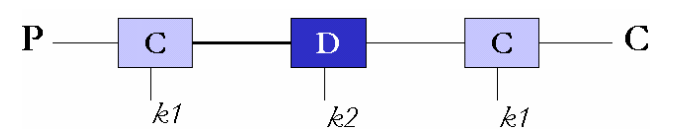
\includegraphics[width=0.5\linewidth]{image.png}
%     \caption{Cifrado de bloque Triple-DES}
%     \label{fig:enter-label}
% \end{figure}
¿Por qué en el modelo de cifrado de bloque de Triple-DES se fortalece el algoritmo a partir del incremento del dominio de la clave y por qué simplemente no se aumenta el tamaño de la misma aplicando una sola vez el algoritmo de cifrado?

\textbf{Respuesta:}

En 3DES se fortalece el algoritmo mediante el incremento del dominio de la clave porque:
\begin{itemize}
    \item Primero que todo aumenta el espacio de claves efectivo sin modificar la estructura básica del algoritmo DES.
    \item Segundo, se tiene una aplicación repetida con diferentes claves para mitigar las vulnerabilidades específicas de DES.
    \item El simple aumento del tamaño de la clave en DES no solucionaría las debilidades estructurales del diseño original.
    \item La arquitectura del DES original está limitada a 56 bits de clave y modificarla para aceptar claves más grandes requeriría rediseñar prácticamente pues todo el algoritmo.
\end{itemize}

\subsection{Literal b}
¿Qué significan las secuencias pseudo-aleatorias en criptografía? ¿Cómo minimizar el riesgo de baja entropía en el cálculo de claves?
\\
\textbf{Respuesta:}

Las secuencias pseudo-aleatorias en criptografía son:
\begin{itemize}
    \item Series de bits generadas por algoritmos deterministas que parecen aleatorias.
    \item Fundamentales para la generación de claves, vectores de inicialización y nonces.
\end{itemize}

Para minimizar el riesgo de baja entropía:
\begin{itemize}
    \item Utilizar fuentes de entropía de alta calidad (ruido térmico, variaciones en hardware, etc.)
    \item Implementar el PRNG criptográficamente seguros (CSPRNG)
    \item Aplicar técnicas de post-procesamiento (función hash) a los datos aleatorios
    \item Realizar pruebas estadísticas de aleatoriedad
\end{itemize}




\subsection{Literal c}
En un cifrador de producto basado en DES/3DES, determine el valor de salida (entero) para la S-Box de la Figura 1, con bloque de entrada 100101, donde $r = b_0b_5$ y $c = b_1b_2b_3b_4$.

\begin{figure}[h]
\centering
\begin{tabular}{|c|c|c|c|c|c|c|c|c|c|c|c|c|c|c|c|c|}
\hline
\multicolumn{17}{|c|}{$S_0$} \\
\hline
& 0 & 1 & 2 & 3 & 4 & 5 & 6 & 7 & 8 & 9 & 10 & 11 & 12 & 13 & 14 & 15 \\
\hline
0 & 14 & 4 & 13 & 1 & 2 & 15 & 11 & 8 & 3 & 10 & 6 & 12 & 5 & 9 & 0 & 7 \\
\hline
1 & 0 & 15 & 7 & 4 & 14 & 2 & 13 & 1 & 10 & 6 & 12 & 11 & 9 & 5 & 3 & 8 \\
\hline
2 & 4 & 1 & 14 & 8 & 13 & 6 & 2 & 11 & 15 & 12 & 9 & 7 & 3 & 10 & 5 & 0 \\
\hline
3 & 15 & 12 & 8 & 2 & 4 & 9 & 1 & 7 & 5 & 11 & 3 & 14 & 10 & 0 & 6 & 13 \\
\hline
\end{tabular}
\caption{S-Box $S_0$ para el cifrador DES}
\end{figure}

\textbf{Solución:}

Tenemos que entonces el bloque de entrada es $100101$

Según el enunciado:
\begin{itemize}
    \item $r = b_0b_5 = (1~1) = 11_2 = 3_{10}$ (la fila 3)
    \item $c = b_1b_2b_3b_4 = (0~0~1~0) = 0010_2 = 2_{10}$ (columna 2)
\end{itemize}

Para obtener el valor de salida, debemos consultar la S-Box $S_0$ en la intersección de la fila 3 y la columna 2:

$$
\begin{array}{|c|c|c|}
\hline
\text{Fila } r & \text{Columna } c & \text{Valor} \\
\hline
3 & 2 & 8 \\
\hline
\end{array}
$$

Por lo tanto el valor que tenemos en la salida (entero) para la S-Box con la entrada $100101$ es 8.


\section{Problema 4 (25\%)}



\subsection{Literal a}
Explique (en pseudo-código) cómo puede implementarse un algoritmo de cifrado de bloque que use mecanismos de sustitución, permutación y condiciones iniciales "fuertes", cálculo de claves. No es necesario ajustarse a estándares ya existentes.

\textbf{Solución}

Para implementar un algoritmo de cifrado por bloques robusto, se requieren varios componentes fundamentales que cumplen propósitos específicos:

\begin{itemize}
    \item \textbf{Entrada y salida}: Mensaje original $M$ y clave secreta $K$ como entradas, texto cifrado $C$ como salida.
    
    \item \textbf{Generación de subclaves}: Derivamos múltiples subclaves a partir de la clave principal porque hay que aumentar la complejidad criptográfica y dificultar ataques de criptoanálisis.
    
    \item \textbf{Condiciones iniciales fuertes}: Aplicamos una permutación inicial para dispersar los bits del mensaje para asegurar que pequeños cambios en la entrada afecten inmediatamente a todo el bloque.
    
    \item \textbf{Proceso de rondas}: Aplicamos múltiples iteraciones de transformaciones para lograr una fuerte difusión y confusión:
        \begin{itemize}
            \item \textbf{Expansión}: Aumentamos el tamaño del estado para crear redundancia y ampliar la superficie de operación.
            
            \item \textbf{Mezcla con subclave}: Combinamos mediante XOR para integrar la información de la clave con el estado actual, creando dependencia de la clave en cada ronda.
            
            \item \textbf{Sustitución}: Aplicamos S-Boxes para introducir no-linealidad, crucial para resistir ataques de criptoanálisis lineal.
            
            \item \textbf{Permutación}: Redistribuimos los bits para garantizar que los cambios en una parte afecten rápidamente a todo el bloque en las siguientes rondas.
        \end{itemize}
\end{itemize}

\textbf{\textit{Pseudo-código:}}

\begin{lstlisting}[basicstyle=\ttfamily\small]
Algoritmo CifradoBloque:
    Entrada: Mensaje M, Clave K
    Salida: Texto cifrado C
    
    // Generación de sub-claves
    SubClaves = GenerarSubClaves(K, NumeroRondas)
    
    // Condiciones iniciales
    EstadoInicial = AplicarPermutacionInicial(M)
    
    // Proceso de rondas
    Estado = EstadoInicial
    Para i desde 1 hasta NumeroRondas:
        // Expansión
        EstadoExpandido = Expansion(Estado)
        
        // Mezcla con subclave
        EstadoMezclado = XOR(EstadoExpandido, SubClaves[i])
        
        // Sustitución (S-Boxes)
        EstadoSustituido = AplicarSustituciones(EstadoMezclado)
        
        // Permutación
        Si i < NumeroRondas entonces:
            Estado = AplicarPermutacion(EstadoSustituido)
        Sino:
            Estado = EstadoSustituido
        Fin Si
    Fin Para
    
    // Permutación final
    C = AplicarPermutacionFinal(Estado)
    
    Retornar C
Fin Algoritmo
\end{lstlisting}

Las funciones auxiliares se implementarían de la siguiente manera:

\begin{itemize}
    \item \textbf{GenerarSubClaves}: Deriva múltiples claves a partir de la clave principal mediante rotaciones, permutaciones y selecciones de bits, garantizando que cada ronda utilice material criptográfico distinto.
    
    \item \textbf{AplicarPermutacionInicial}: Reorganiza los bits del mensaje según una tabla predefinida para asegurar una distribución inicial óptima.
    
    \item \textbf{Expansion}: Aumenta el tamaño del bloque mediante duplicación selectiva de bits para crear más puntos de interacción con la subclave.
    
    \item \textbf{AplicarSustituciones}: Transforma grupos de bits utilizando tablas no lineales (S-Boxes) que mapean entradas a salidas de forma que resistan análisis diferencial y lineal.
    
    \item \textbf{AplicarPermutacion}: Redistribuye los bits resultantes para maximizar el efecto avalancha, donde un cambio en un bit de entrada afecta aproximadamente la mitad de los bits de salida.
    
    \item \textbf{AplicarPermutacionFinal}: Realiza una última reorganización de bits, típicamente inversa a la permutación inicial, para finalizar el proceso de cifrado.
\end{itemize}

La fortaleza de este diseño radica en la combinación de múltiples capas de transformaciones no lineales (sustituciones) con transformaciones lineales (permutaciones), aplicadas repetidamente para crear un cifrado resistente a diversas técnicas de criptoanálisis.





\subsection{Literal b}
Describa brevemente los principales métodos de sustitución y permutación del algoritmo AES/Rijndael e infiera por qué es el estándar de cifrado simétrico más robusto en estos tiempos.
\\
\textbf{Respuesta:}
El algoritmo AES (Advanced Encryption Standard) desarrollado por Vincent Rijmen y Joan Daemen \textit{(basado en Rijndael)}, se estructura en un proceso de cifrado por rondas con operaciones específicas que garantizan tanto la confusión como la difusión de la información. A diferencia de los predecesores como DES, AES no utiliza una estructura Feistel, sino una arquitectura basada en sustitución-permutación (SP) que opera sobre una matriz de estado de 4×4 bytes.

\textbf{Principales métodos de sustitución y permutación en AES:}

\begin{itemize}
    \item \textbf{SubBytes (Sustitución)}: Transformación no lineal que sustituye cada byte del estado por otro valor según una tabla S-Box predefinida. Esta operación:
    \begin{itemize}
        \item Proporciona la no-linealidad necesaria para resistir ataques de criptoanálisis lineal.
        \item Está diseñada matemáticamente para minimizar correlaciones entre bits de entrada y salida.
        \item Se implementa como la inversión en el campo finito GF(2$^8$) seguida de una transformación afín.
    \end{itemize}
    
    \item \textbf{ShiftRows (Permutación)}: Operación donde cada fila de la matriz de estado se desplaza cíclicamente un número diferente de posiciones:
    \begin{itemize}
        \item La primera fila no se desplaza.
        \item La segunda fila se desplaza 1 byte hacia la izquierda.
        \item La tercera fila se desplaza 2 bytes hacia la izquierda.
        \item La cuarta fila se desplaza 3 bytes hacia la izquierda.
        \item Asegura que los bytes de cada columna se dispersen a diferentes columnas, contribuyendo a la difusión entre columnas.
    \end{itemize}
    
    \item \textbf{MixColumns (Difusión)}: Transformación lineal que opera sobre las columnas de la matriz de estado:
    \begin{itemize}
        \item Cada columna se trata como un polinomio de cuatro términos en GF(2$^8$).
        \item Se multiplica módulo $x^4+1$ con un polinomio fijo $a(x) = \{03\}x^3 + \{01\}x^2 + \{01\}x + \{02\}$.
        \item Garantiza que cada byte de salida dependa de todos los bytes de entrada de esa columna.
        \item Proporciona difusión a nivel de columna, complementando la difusión entre columnas de ShiftRows.
    \end{itemize}
    
    \item \textbf{AddRoundKey (Combinación)}: Operación que combina mediante XOR el estado actual con la subclave de ronda:
    \begin{itemize}
        \item Incorpora material de la clave en cada ronda.
        \item Es la única operación que utiliza la clave, proporcionando la seguridad del cifrado.
        \item Simple pero efectiva debido a las propiedades matemáticas del XOR.
    \end{itemize}
\end{itemize}

\textbf{Estructura de rondas en AES:}
\begin{itemize}
    \item \textbf{Ronda inicial}: Aplica únicamente AddRoundKey con la clave original.
    \item \textbf{Rondas principales}: Aplica secuencialmente SubBytes, ShiftRows, MixColumns y AddRoundKey (con 9 rondas para AES-128).
    \item \textbf{Ronda final}: Aplica SubBytes, ShiftRows y AddRoundKey (omite MixColumns).
\end{itemize}

\textbf{AES es considerado el estándar más robusto actualmente porque tiene:}
\begin{itemize}
    \item \textbf{Diseño matemático riguroso}: Basado en principios algebraicos sólidos en campos finitos GF(2$^8$), que proporcionan propiedades criptográficas óptimas.
    
    \item \textbf{Arquitectura innovadora}: A diferencia de los cifradores Feistel tradicionales (como DES, Lucifer, Blowfish), AES procesa el bloque completo en cada ronda, aumentando la difusión y confusión.
    
    \item \textbf{Flexibilidad y escalabilidad}: Permite tamaños de clave de 128, 192 y 256 bits, adaptándose a diferentes requisitos de seguridad y resistiendo ataques cuánticos futuros con claves de mayor longitud.
    
    \item \textbf{Eficiencia computacional}: Diseñado específicamente para optimizar el rendimiento tanto en implementaciones hardware (tarjetas inteligentes con procesadores de 8 bits) como en software (CPUs de 32 bits).
    
    \item \textbf{Resistencia probada}: Ha resistido más de dos décadas de intenso análisis criptográfico sin vulnerabilidades prácticas, mientras que sus contemporáneos como RC2, CAST y IDEA han mostrado debilidades significativas.
    
    \item \textbf{Ausencia de puertas traseras}: A diferencia de algunos algoritmos como Skipjack (propuesto para comunicaciones oficiales en EE.UU.), AES fue seleccionado tras un concurso público abierto y transparente, sin componentes secretos o sospechosos.
    
    \item \textbf{Balance óptimo entre seguridad y rendimiento}: Proporciona un alto nivel de seguridad con una eficiencia computacional excepcional, permitiendo su implementación en dispositivos con recursos limitados.
\end{itemize}

La robustez de AES radica principalmente en su capacidad para crear una fuerte difusión (donde un cambio en un bit de entrada afecta a múltiples bits de salida) y confusión (donde la relación entre la clave y el texto cifrado es compleja), principios fundamentales establecidos por Claude Shannon. Su combinación única de operaciones algebraicas, estructura de rondas y manejo de bytes como elementos de un campo finito lo convierten en un algoritmo matemáticamente sólido y prácticamente invulnerable a los ataques criptoanalíticos conocidos.




\subsection{Literal c}
¿Por qué la operación XOR es usada en los algoritmos criptográficos que operan a nivel de bit y de byte? De un ejemplo.

\textbf{Respuesta:}
La operación XOR (OR exclusivo) es fundamental en algoritmos criptográficos por sus propiedades matemáticas y prácticas:

\begin{itemize}
    \item \textbf{Propiedad de inversión:} $A \oplus B \oplus B = A$ - Esta propiedad permite cifrar y descifrar con la misma operación.
    
    \item \textbf{Distribución uniforme:} Cuando se aplica XOR entre un texto y una clave verdaderamente aleatoria, el resultado no revela patrones estadísticos del texto original.
    
    \item \textbf{Eficiencia computacional:} La operación XOR se implementa con un solo ciclo de reloj en hardware, siendo extremadamente rápida.
    
    \item \textbf{Neutralidad estadística:} No introduce sesgo en la distribución de bits del resultado cuando se aplica con valores aleatorios.
    
    \item \textbf{Propiedad conmutativa:} $A \oplus B = B \oplus A$ - El orden de los operandos no altera el resultado.
\end{itemize}

\textbf{Ejemplo práctico con caracteres ASCII:}

Vamos a cifrar la palabra \texttt{CINCO} usando la clave \texttt{CLAVE} mediante XOR a nivel de byte:

\begin{center}
\begin{tabular}{|c|c|c|c|c|c|}
\hline
\textbf{Operación / Caracter} & \textbf{1} & \textbf{2} & \textbf{3} & \textbf{4} & \textbf{5} \\
\hline

\textbf{Cinco (ASCII)} & \textbf{C} (67) & \textbf{I} (73) & \textbf{N} (78) & \textbf{C} (67) & \textbf{O} (79) \\
\hline
% \textbf{Texto plano (ASCII)} &  \\
% \hline
\textbf{Cinco (binario)} & 01000011 & 01001001 & 01001110 & 01000011 & 01001111 \\
\hline
\textbf{Clave (ASCII)} & C (67) & L (76) & A (65) & V (86) & E (69) \\
\hline
\textbf{Clave (binario)} & 01000011 & 01001100 & 01000001 & 01010110 & 01000101 \\
\hline
\textbf{Cinco XOR Clave} & 00000000 & 00000101 & 00001111 & 00010101 & 00001010 \\
% \hline
% \textbf{Texto cifrado (decimal)} & 0 & 5 & 15 & 21 & 10 \\
% \hline
% \textbf{Texto cifrado (carácter)} & NUL & ENQ & SI & NAK & LF \\
\hline
\end{tabular}
\end{center}

\textbf{Proceso de descifrado:}

Para recuperar el texto original pues aplicamos nuevamente la operación XOR con la misma clave:

\begin{center}
\begin{tabular}{|c|c|c|c|c|c|}
\hline
\textbf{Operación / Caracter} & \textbf{1} & \textbf{2} & \textbf{3} & \textbf{4} & \textbf{5} \\
\hline
% \textbf{Texto cifrado (decimal)} & 0 & 5 & 15 & 21 & 10 \\
% \hline
\textbf{Texto cifrado (binario)} & 00000000 & 00000101 & 00001111 & 00010101 & 00001010 \\
\hline
\textbf{Clave (ASCII)} & C (67) & L (76) & A (65) & V (86) & E (69) \\
\hline
\textbf{Clave (binario)} & 01000011 & 01001100 & 01000001 & 01010110 & 01000101 \\
\hline
\textbf{XOR resultante (binario)} & 01000011 & 01001001 & 01001110 & 01000011 & 01001111 \\
\hline
\textbf{Texto recuperado (decimal)} & 67 & 73 & 78 & 67 & 79 \\
\hline
\textbf{Texto recuperado (carácter)} & C & I & N & C & O \\
\hline
\end{tabular}
\end{center}

\textbf{Demostración de propiedades clave:}

En este ejemplo podemos observar varias propiedades importantes:

\begin{enumerate}
    \item \textbf{Inversión perfecta:} El primer carácter 'C' con valor ASCII 67 se cifra con su homólogo en la clave (también 'C' con valor 67), lo que resulta en 0 (NUL). Esta equivalencia demuestra cómo dos valores idénticos al aplicar XOR se anulan completamente.
    
    \item \textbf{No correlación:} Caracteres similares en el texto plano (las dos 'C' en CINCO) producen diferentes resultados cifrados (0 y 21) debido a las diferentes letras de la clave en esas posiciones ('C' y 'V').
    
    \item \textbf{Difusión:} Un solo bit diferente entre el texto y la clave puede cambiar aproximadamente la mitad de los bits del resultado.
\end{enumerate}

El ejemplo busca mostrar por qué esta operación XOR es el fundamento de muchas primitivas criptográficas, desde el cifrado básico one-time pad hasta operaciones más complejas en cifrados por bloques como AES, donde se utiliza en la fase AddRoundKey para combinar el estado con la subclave de ronda.




% \pagebreak
\subsection*{Muchas gracias por la atención.\\Over V.}

}